% Auto-generated by r_project/simulation/mc_paper.R
% Generated 2026-11-26 17:24 at commit 24c7f52 (uncommitted changes)
% Monte Carlo rows: commit(s) 7acc201, 2ae035d, f3382b0, bd2f334, 9ceeb42, c1a3c0b, 94dfe82, f1ebed4, 9e7ae33, 24c7f52; targets: commit f3382b0,9ceeb42,c1a3c0b,94dfe82,f1ebed4,bd2f334,24c7f52,9e7ae33,817ab68

\begin{figure}[htbp]
\centering
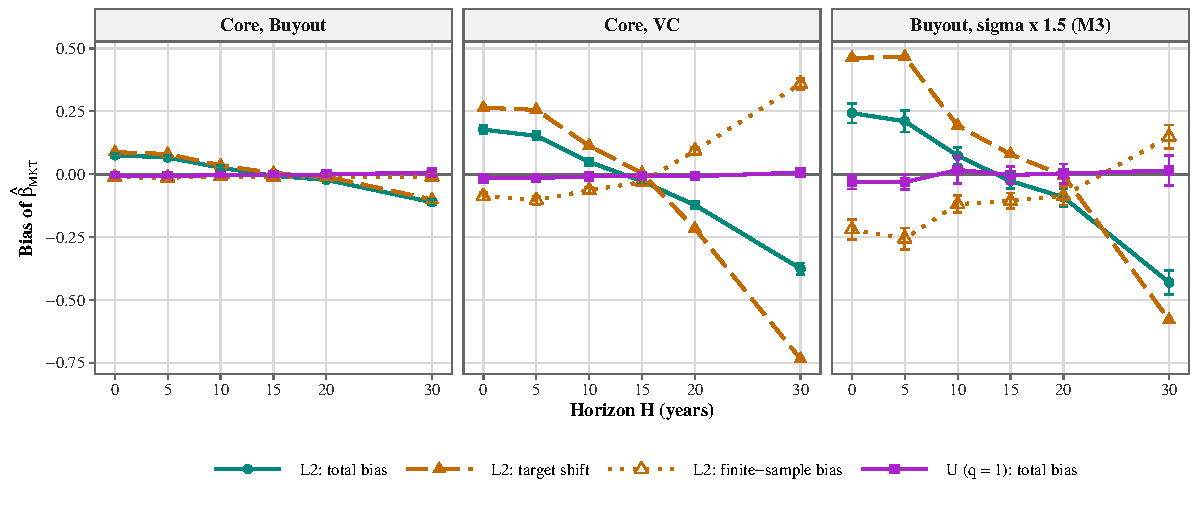
\includegraphics[width=\textwidth]{figure_S1_decomposition.pdf}
\caption{Monte Carlo: where the bias of L2 comes from}
\label{fig:mc_decomposition}
\par\vspace{2pt}
{\scriptsize\textit{Notes:} Bias of the single-factor $\hat\beta_{MKT}$ (true value 1) by horizon. L2 on vintage portfolios is split into the target shift (the minimizer of the criterion averaged over replications 1--200, minus the true value; T3/T4) and the finite-sample bias (mean estimate minus that target). $U_{v,H}$ with $q_v=1$ for comparison; its target is the true value (T7). Bars: $\pm2$ Monte Carlo SE of the mean estimate; the target's own Monte Carlo precision (half the difference between replications 1--100 and 101--200) is 0.002--0.011 at 0--20 years, 0.009 at 30 years (Buyout) and 0.006--0.035 at 0--20 years, 0.106 at 30 years (VC), not estimated for M3. Core designs as in Table~\ref{tab:mc_core} (1{,}000 replications); M3: Buyout core with $1.5\times$ the calibrated $\sigma$ (250 replications).}
\end{figure}
